\documentclass[11pt]{article}
\usepackage[margin=1in]{geometry}
\usepackage{graphicx}
\usepackage{booktabs}
\usepackage{longtable}
\usepackage{array}
\usepackage{float}
\usepackage{caption}
\usepackage{subcaption}
\usepackage{xcolor}
\usepackage{hyperref}
\usepackage{amsmath}
\usepackage{placeins}
\hypersetup{colorlinks=true,linkcolor=blue!50!black,urlcolor=blue!50!black,citecolor=blue!50!black}
\graphicspath{{figures/}}
\title{Multivariate Analysis of the Doubs River Fish-Environment System}
\author{Generated from the BCB743 Quantitative Ecology data}
\date{07 July 2026}
\begin{document}
\maketitle
\begin{abstract}
The Doubs River fish and environmental data were analysed with the main multivariate methods of the Quantitative Ecology chapters, namely PCA, CA, DCA, PCoA, nMDS, RDA, CCA, and db-RDA, and then extended with variable-selection, spatial, beta-diversity, and species-response analyses. The methods agree on one dominant structure, a longitudinal river-continuum gradient from cool, steep, oxygen-rich headwaters to lower, slower, nutrient- and organic-load-enriched reaches, and fish composition follows it as an ordered replacement of trout-zone species by lowland cyprinids. Two refinements emerge from the extended analyses. A short mid-river reach departs from the continuum as an organic-pollution oxygen sag that collapses local richness and keeps oxygen and biological oxygen demand in the selected models, and the contrast between data-driven and theory-driven variable selection shows that the retained oxygen variables are proximate correlates of an upstream nutrient load rather than independent causes. Constrained models explain about half of the community variation, and beta-diversity partitioning attributes most of the turnover to species replacement.
\end{abstract}
\section{Data and Pre-processing}
The source files are the local BCB743 Doubs River tables. Environmental PCA used all 30 environmental rows. Species ordinations and constrained analyses removed site 8 because it has zero total fish abundance, which leaves 29 matched fish, environmental, and spatial rows.
\begin{table}[!h]
\centering
\caption{\label{tab:tab:data-overview}Local Doubs River data files used in this report.}
\centering
\resizebox{\ifdim\width>\linewidth\linewidth\else\width\fi}{!}{
\fontsize{8}{10}\selectfont
\begin{tabular}[t]{lllll}
\toprule
Table & Role & Rows & Columns & Notes\\
\midrule
DoubsEnv.csv & Environmental predictors & 30 & 11 & Used for PCA; matched subset used for direct gradient analyses\\
DoubsSpe.csv & Fish abundance response & 30 & 27 & Site 8 has zero total abundance and was removed for species ordinations\\
DoubsSpa.csv & Spatial coordinates & 30 & 2 & Used for the site map\\
\bottomrule
\end{tabular}}
\end{table}
\begin{table}[!h]
\centering
\caption{\label{tab:tab:env-summary}Environmental variables and their longitudinal behaviour. The last column is the Pearson correlation with distance from source (`dfs`) across all 30 sites.}
\centering
\resizebox{\ifdim\width>\linewidth\linewidth\else\width\fi}{!}{
\fontsize{7}{9}\selectfont
\begin{tabular}[t]{llllll}
\toprule
Code & Variable & Minimum & Median & Maximum & r with dfs\\
\midrule
\texttt{dfs} & Distance from source & 0.30 & 175.20 & 453.00 & 1.00\\
\texttt{alt} & Altitude & 172.00 & 395.00 & 934.00 & -0.94\\
\texttt{slo} & Channel slope & 0.20 & 1.20 & 48.00 & -0.38\\
\texttt{flo} & Flow rate & 0.84 & 22.10 & 69.00 & 0.95\\
\texttt{pH} & pH & 7.70 & 8.00 & 8.60 & 0.01\\
\texttt{har} & Water hardness & 40.00 & 89.00 & 110.00 & 0.70\\
\texttt{pho} & Phosphate & 0.01 & 0.29 & 4.22 & 0.48\\
\texttt{nit} & Nitrate & 0.15 & 1.60 & 6.20 & 0.75\\
\texttt{amm} & Ammonium & 0.00 & 0.10 & 1.80 & 0.41\\
\texttt{oxy} & Dissolved oxygen & 4.10 & 10.20 & 12.40 & -0.51\\
\texttt{bod} & Biological oxygen demand & 1.30 & 4.15 & 16.70 & 0.39\\
\bottomrule
\end{tabular}}
\end{table}
\begin{figure}[H]
\centering
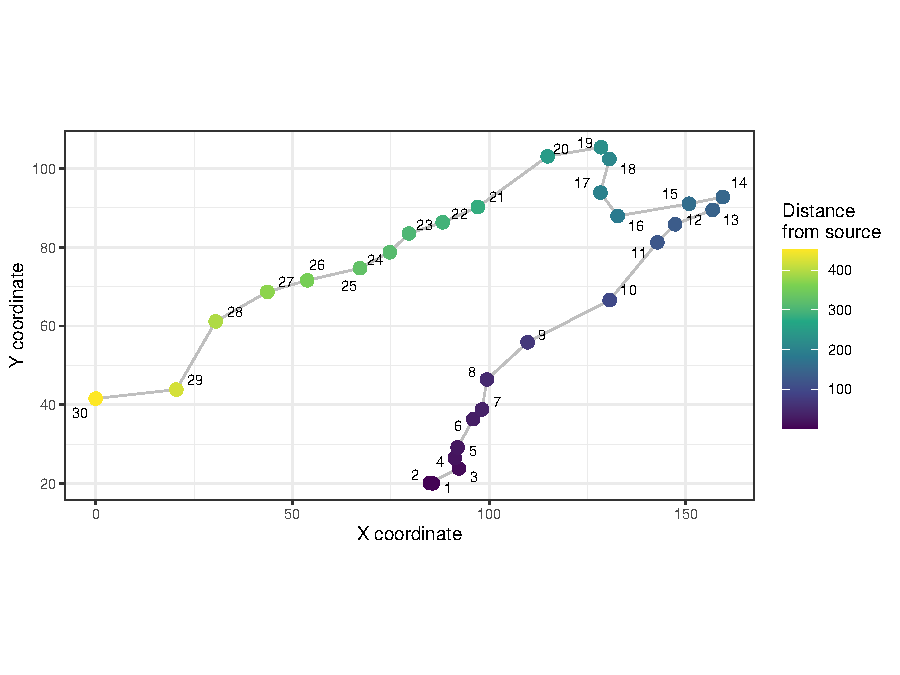
\includegraphics[width=0.78\linewidth]{fig01_doubs_sites.pdf}
\caption{Spatial configuration of the Doubs River sites. Colour gives distance from source.}
\label{fig:sites}
\end{figure}
\section{Methods}
The methods follow the BCB743 ordination sequence and then extend it with a set of more advanced checks, each asking a sharper question of the same data. Unconstrained ordinations come first. They let the data reveal their dominant structure without forcing environmental predictors into the solution. PCA summarises covariance among the measured environmental variables, CA and DCA summarise unimodal fish turnover, and PCoA and nMDS summarise Bray-Curtis dissimilarities among sites. Constrained ordinations come second, and they ask a sharper question, namely how much of the fish-composition pattern the measured environmental variables can account for. RDA, CCA, and db-RDA answer that question under three different geometries. The advanced analyses come last. They ask whether the same conclusion survives when the problem is reframed in terms of collinearity, spatial structure, distributional assumptions, the philosophy of variable selection, and the shape of individual species responses.
\begin{table}[!h]
\centering
\caption{\label{tab:tab:method-summary}Summary of methods and headline outputs.}
\centering
\resizebox{\ifdim\width>\linewidth\linewidth\else\width\fi}{!}{
\fontsize{7}{9}\selectfont
\begin{tabular}[t]{llll}
\toprule
Method & Response & Key output & Interpretation\\
\midrule
PCA & 11 environmental variables & PC1 = 54.3\%, PC2 = 19.7\% & Environmental covariance forms a strong river-continuum axis.\\
CA & 27 fish abundance columns & CA1 = 51.5\%, CA2 = 12.4\% & Species composition turns over mainly along the river continuum.\\
DCA & 27 fish abundance columns & DCA1 axis length = 3.86 & Gradient length supports a long unimodal species gradient and explains the CA arch.\\
PCoA & Bray-Curtis dissimilarity of fish assemblages & MDS1 = 52.4\% of positive inertia & Bray-Curtis distances recover the same faunal turnover.\\
nMDS & Ranks of Bray-Curtis dissimilarities & Stress = 0.075 & Rank-order composition has a faithful two-dimensional representation.\\
RDA & Hellinger-transformed fish abundances & Selected: dfs, oxy, bod; adj. $R^2$ = 0.54 & Linear constrained model confirms environment-composition coupling.\\
CCA & Raw fish abundance table & Selected: dfs, oxy, alt; adj. $R^2$ = 0.50 & Unimodal constrained model confirms the same coupling.\\
db-RDA & Bray-Curtis dissimilarity of fish assemblages & Selected: dfs, bod, oxy; adj. $R^2$ = 0.57 & Distance-based constrained model gives the clearest community-distance test.\\
\bottomrule
\end{tabular}}
\end{table}
\section{Unconstrained Gradients}
\subsection{Environmental PCA}
The standardised environmental PCA is strongly one-dimensional: PC1 explains 54.3\% of the environmental variance and PC2 explains 19.7\%. PC1 contrasts high-altitude, high-oxygen, steep upper sites against downstream sites with higher distance from source, discharge, nitrate, phosphate, ammonium, hardness, and biological oxygen demand.
\begin{table}[!h]
\centering
\caption{\label{tab:tab:pca-eig}Environmental PCA eigenvalues.}
\centering
\resizebox{\ifdim\width>\linewidth\linewidth\else\width\fi}{!}{
\fontsize{8}{10}\selectfont
\begin{tabular}[t]{llll}
\toprule
Axis & Eigenvalue & Percent & Cumulative\\
\midrule
PC1 & 5.9687 & 54.26 & 54.26\\
PC2 & 2.1639 & 19.67 & 73.93\\
PC3 & 1.0652 & 9.68 & 83.62\\
PC4 & 0.7388 & 6.72 & 90.33\\
PC5 & 0.4002 & 3.64 & 93.97\\
PC6 & 0.3356 & 3.05 & 97.02\\
\bottomrule
\end{tabular}}
\end{table}
\begin{table}[!h]
\centering
\caption{\label{tab:tab:pca-load}Environmental PCA variable scores, sorted by absolute PC1 loading.}
\centering
\resizebox{\ifdim\width>\linewidth\linewidth\else\width\fi}{!}{
\fontsize{8}{10}\selectfont
\begin{tabular}[t]{llll}
\toprule
Code & Variable & PC1 & PC2\\
\midrule
\texttt{nit} & Nitrate & 1.150 & -0.100\\
\texttt{dfs} & Distance from source & 1.087 & 0.534\\
\texttt{pho} & Phosphate & 1.058 & -0.601\\
\texttt{alt} & Altitude & -1.044 & -0.615\\
\texttt{amm} & Ammonium & 1.007 & -0.697\\
\texttt{oxy} & Dissolved oxygen & -0.975 & 0.499\\
\texttt{bod} & Biological oxygen demand & 0.973 & -0.715\\
\texttt{flo} & Flow rate & 0.958 & 0.661\\
\texttt{har} & Water hardness & 0.901 & 0.585\\
\texttt{slo} & Channel slope & -0.577 & -0.489\\
\texttt{pH} & pH & -0.064 & 0.463\\
\bottomrule
\end{tabular}}
\end{table}
\begin{figure}[H]
\centering
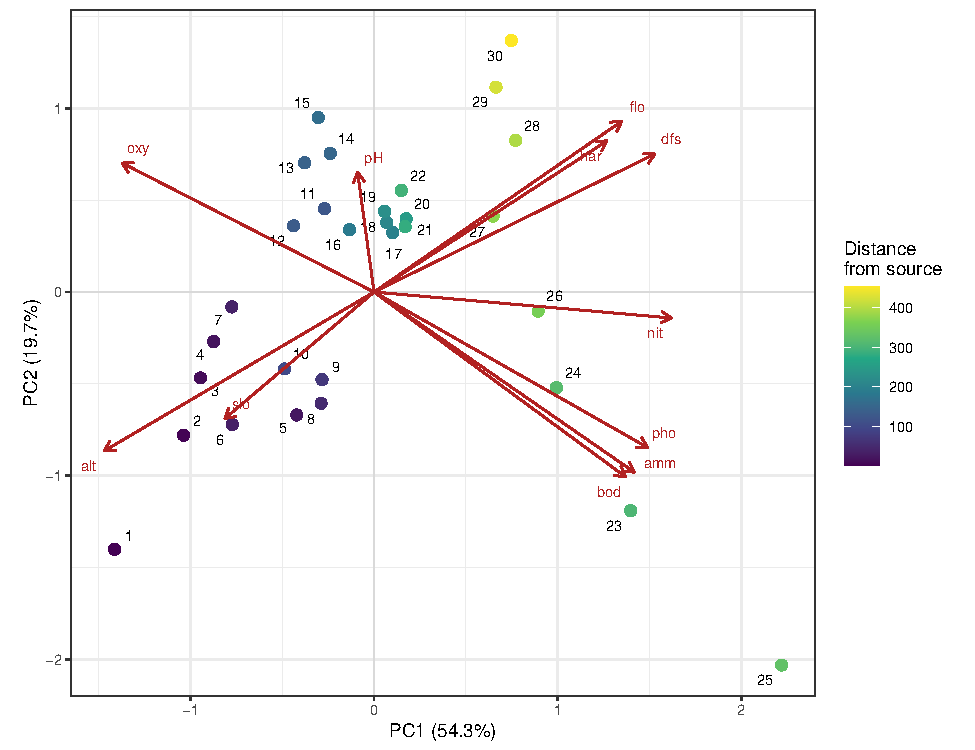
\includegraphics[width=0.82\linewidth]{fig02_environmental_pca.pdf}
\caption{PCA biplot of the Doubs environmental variables. Arrows indicate environmental loadings; sites are coloured by distance from source.}
\label{fig:pca}
\end{figure}
\subsection{Species CA and DCA}
CA gives the same gradient through the fish assemblage. CA1 explains 51.5\% of total inertia and CA2 explains 12.4\%. DCA estimates the first gradient length as 3.86 standard deviation units, which is long enough for clear species turnover and explains why a CA arch appears on the second axis.
\begin{table}[!h]
\centering
\caption{\label{tab:tab:ca-eig}Correspondence analysis eigenvalues.}
\centering
\resizebox{\ifdim\width>\linewidth\linewidth\else\width\fi}{!}{
\fontsize{8}{10}\selectfont
\begin{tabular}[t]{llll}
\toprule
Axis & Eigenvalue & Percent & Cumulative\\
\midrule
CA1 & 0.6010 & 51.50 & 51.50\\
CA2 & 0.1444 & 12.37 & 63.87\\
CA3 & 0.1073 & 9.19 & 73.07\\
CA4 & 0.0834 & 7.14 & 80.21\\
CA5 & 0.0516 & 4.42 & 84.63\\
CA6 & 0.0418 & 3.59 & 88.22\\
\bottomrule
\end{tabular}}
\end{table}
\begin{figure}[H]
\centering
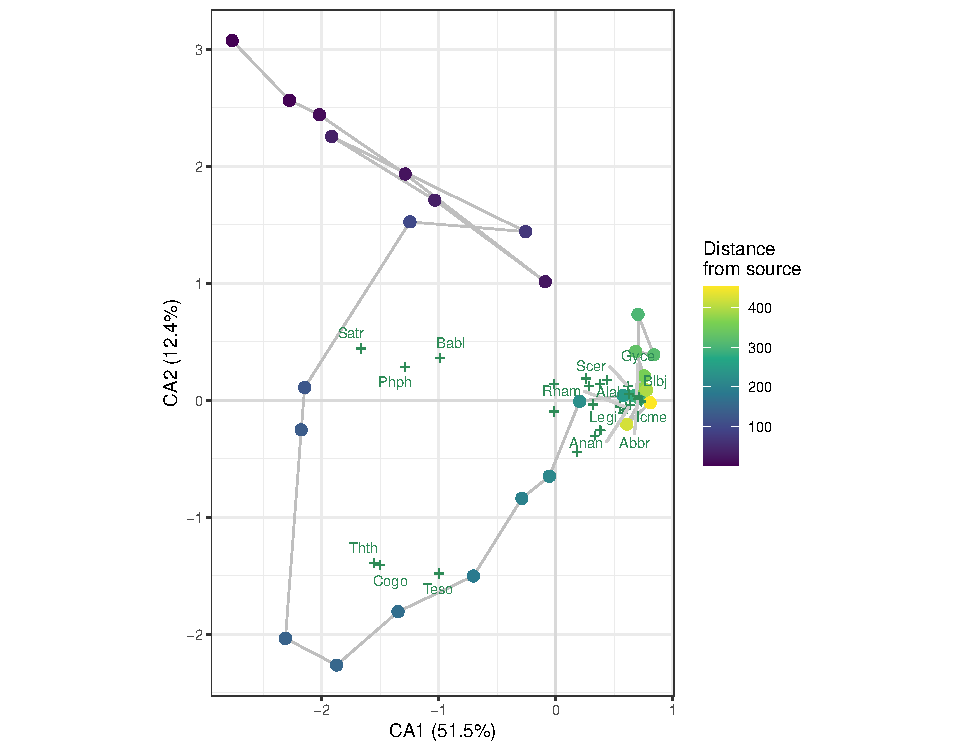
\includegraphics[width=0.82\linewidth]{fig03_species_ca.pdf}
\caption{CA of Doubs fish abundances. Species labels are shown for the more peripheral taxa; points are sites coloured by distance from source.}
\label{fig:ca}
\end{figure}
\begin{figure}[H]
\centering
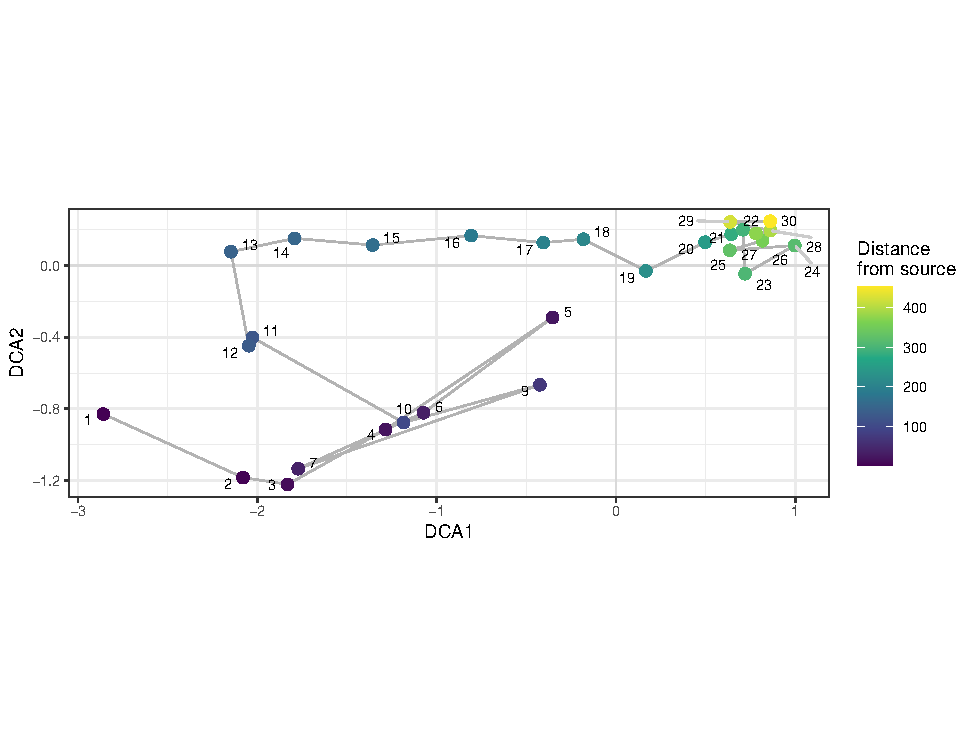
\includegraphics[width=0.78\linewidth]{fig05_dca_gradient.pdf}
\caption{DCA of the Doubs fish data. The connected site sequence shows the long compositional gradient from source to lower reaches.}
\label{fig:dca}
\end{figure}
\subsection{PCoA and nMDS}
The distance-based ordinations recover the same gradient under a geometry free of the CA arch. Bray-Curtis PCoA MDS1 explains 52.4\% of positive inertia, and the nMDS stress is 0.075, a good two-dimensional representation of the rank-order dissimilarities.
\begin{table}[!h]
\centering
\caption{\label{tab:tab:pcoa-eig}PCoA positive eigenvalues for Bray-Curtis fish dissimilarities. Percentages are relative to the sum of positive eigenvalues.}
\centering
\resizebox{\ifdim\width>\linewidth\linewidth\else\width\fi}{!}{
\fontsize{8}{10}\selectfont
\begin{tabular}[t]{llll}
\toprule
Axis & Eigenvalue & Percent & Cumulative\\
\midrule
MDS1 & 3.6953 & 52.35 & 52.35\\
MDS2 & 1.0985 & 15.56 & 67.92\\
MDS3 & 0.7105 & 10.07 & 77.98\\
MDS4 & 0.4150 & 5.88 & 83.86\\
MDS5 & 0.3046 & 4.31 & 88.18\\
MDS6 & 0.1918 & 2.72 & 90.89\\
\bottomrule
\end{tabular}}
\end{table}
Table~\ref{tab:tab:gradient-align} links the ordination figures to the ecological interpretation. For each unconstrained ordination it takes the site scores on the first axis and correlates them with distance from source, the one variable that orders the sites unambiguously from headwater to lower reach. The correlations are alignment diagnostics rather than model tests, since distance from source is fitted in none of these ordinations. It is projected onto them afterwards. A high value therefore says that an axis extracted from the data alone, whether from environmental covariance (PCA), fish turnover (CA), or fish dissimilarity (PCoA and nMDS), reconstructs the physical river order without being told to do so. The four correlations lie between 0.81 and 0.85, so the same upstream-to-downstream sequence emerges from every geometry and from both the environmental and the faunal table. The dominant structure is a property of the system, not of any one method.
\begin{table}[!h]
\centering
\caption{\label{tab:tab:gradient-align}Alignment between first ordination axes and the longitudinal river gradient.}
\centering
\resizebox{\ifdim\width>\linewidth\linewidth\else\width\fi}{!}{
\fontsize{8}{10}\selectfont
\begin{tabular}[t]{ll}
\toprule
Ordination & Correlation with distance from source\\
\midrule
PCA PC1 & 0.853\\
CA CA1 & 0.812\\
PCoA MDS1 & 0.847\\
nMDS NMDS1 & 0.853\\
\bottomrule
\end{tabular}}
\end{table}
\begin{figure}[H]
\centering
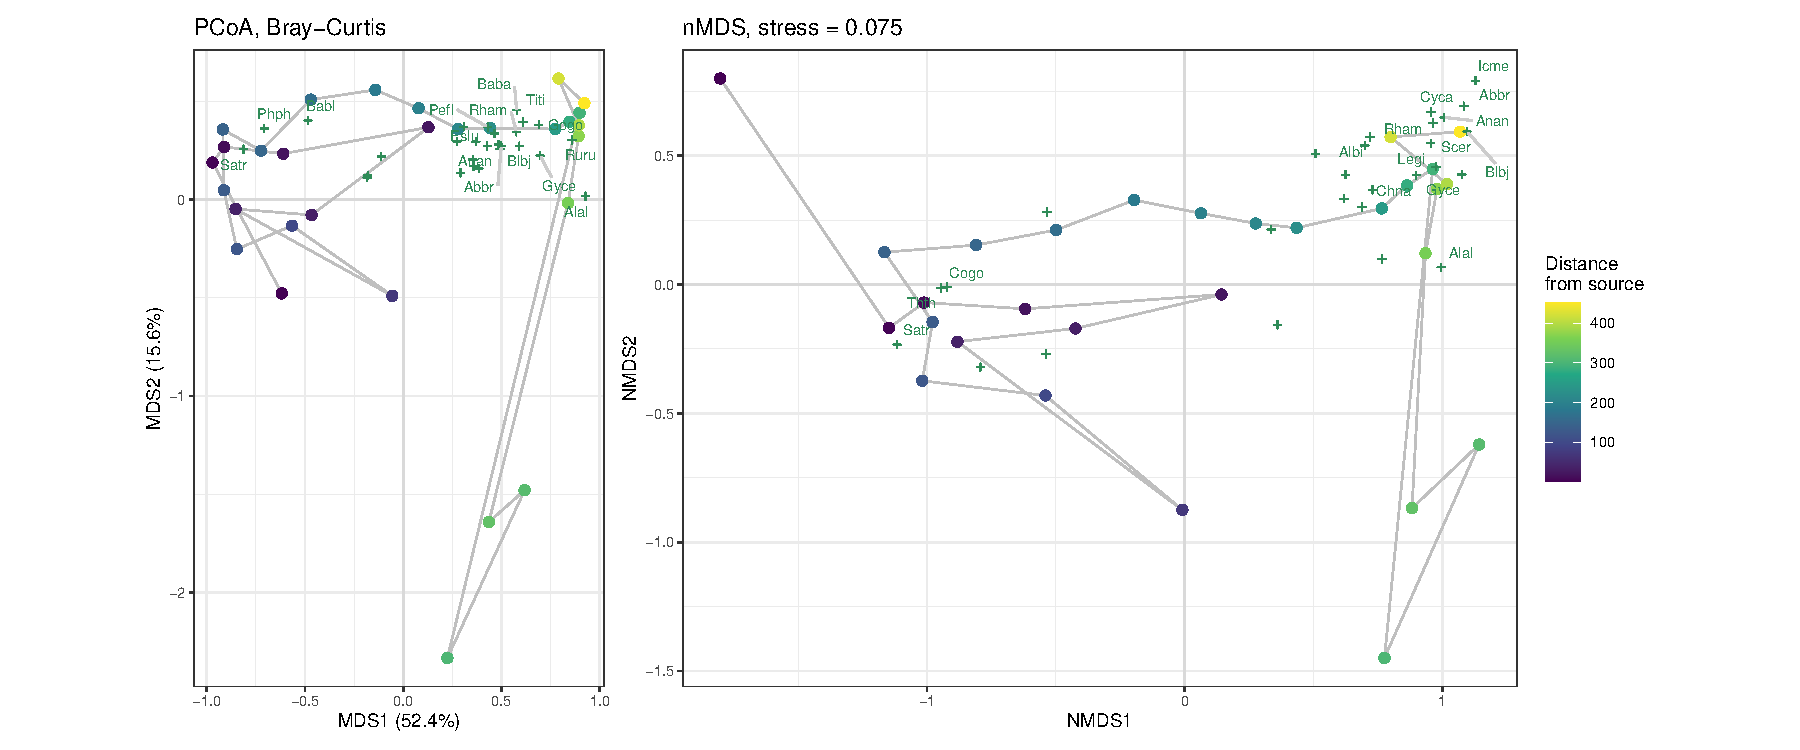
\includegraphics[width=\linewidth]{fig04_pcoa_nmds.pdf}
\caption{Bray-Curtis PCoA and nMDS ordinations of fish composition. Both recover the upstream-to-downstream species gradient.}
\label{fig:pcoa-nmds}
\end{figure}
\subsection{Environmental Vector Fitting}
Vector fitting projects each environmental variable a posteriori onto the CA of fish composition and identifies the variables most aligned with the assemblage pattern. The step is indirect-gradient in character. The CA is built from the fish matrix alone, and the environmental variables enter only afterwards, as arrows fitted to the finished configuration. Table~\ref{tab:tab:ca-envfit} is therefore an interpretation aid and carries none of the inferential weight of a constrained model. Three quantities describe each fitted vector. Its direction gives the part of the ordination in which the variable increases, its $r^2$ gives the strength of association with the two-axis configuration, and its permutation p-value asks whether that association exceeds what random reassignment of the variable to sites would produce. Altitude ($r^2 = 0.81$), distance from source (0.69), and oxygen (0.63) give the longest vectors, followed by hardness, nitrate, and flow. These vectors share a common direction because they express one river-continuum gradient rather than several independent mechanisms. Ammonium, phosphate, and pH fit weakly ($r^2 \leq 0.18$), and two of them fail the permutation test, the first sign that the enrichment variables carry structure the continuum axis does not fully absorb.
\begin{table}[!h]
\centering
\caption{\label{tab:tab:ca-envfit}Environmental vectors fitted to the CA ordination. The $r^2$ column is the squared correlation between the fitted vector and the ordination configuration.}
\centering
\resizebox{\ifdim\width>\linewidth\linewidth\else\width\fi}{!}{
\fontsize{7}{9}\selectfont
\begin{tabular}[t]{llllll}
\toprule
Code & Variable & Axis1 & Axis2 & r2 & p\\
\midrule
\texttt{alt} & Altitude & 0.729 & 0.525 & 0.808 & 0.001\\
\texttt{dfs} & Distance from source & -0.787 & -0.264 & 0.689 & 0.001\\
\texttt{oxy} & Dissolved oxygen & 0.739 & -0.284 & 0.626 & 0.001\\
\texttt{har} & Water hardness & -0.493 & -0.479 & 0.472 & 0.001\\
\texttt{nit} & Nitrate & -0.637 & -0.212 & 0.451 & 0.001\\
\texttt{flo} & Flow rate & -0.619 & -0.248 & 0.444 & 0.001\\
\texttt{slo} & Channel slope & 0.402 & 0.368 & 0.298 & 0.002\\
\texttt{bod} & Biological oxygen demand & -0.445 & 0.160 & 0.224 & 0.036\\
\texttt{pho} & Phosphate & -0.419 & 0.019 & 0.176 & 0.073\\
\texttt{amm} & Ammonium & -0.409 & 0.093 & 0.176 & 0.075\\
\texttt{pH} & pH & 0.153 & -0.260 & 0.091 & 0.231\\
\bottomrule
\end{tabular}}
\end{table}
\begin{figure}[H]
\centering
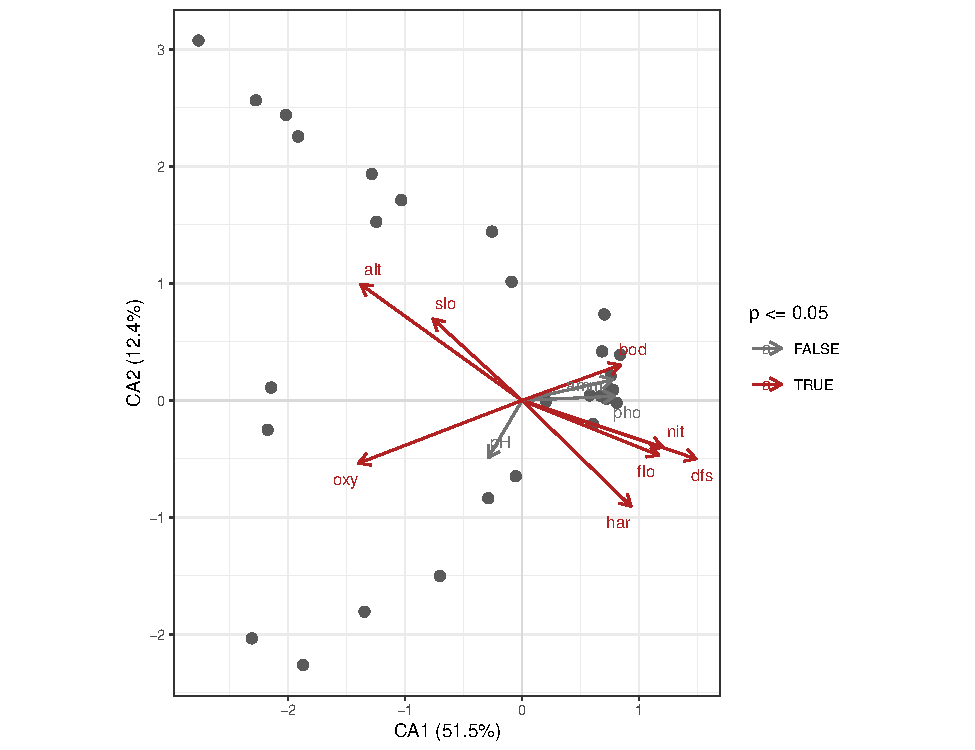
\includegraphics[width=0.82\linewidth]{fig06_ca_envfit.pdf}
\caption{CA ordination with fitted environmental vectors. Red vectors are significant at $p \leq 0.05$.}
\label{fig:envfit}
\end{figure}
\section{Constrained Ordination}
The constrained ordinations ask whether the environmental table explains the fish composition. They are direct-gradient analyses, since the environmental variables build the ordination axes and permutation tests then ask whether the explained component exceeds what chance would produce. This is a stronger statement than vector fitting, though still short of a proof of causation. In a river, many predictors are collinear because altitude, flow, distance from source, oxygen, nutrients, and organic load all change together along the channel. A constrained model can therefore show that the environmental matrix explains community structure while remaining unable to separate the causal contribution of each correlated variable.
Variance inflation factors (VIFs) and forward selection are two diagnostics applied before any interpretation of the selected models. A high VIF marks a variable that is largely predictable from the others, so it cannot be interpreted as an independent effect. Forward selection with \texttt{ordiR2step()} answers a different question. It starts from a null model, tries the candidate variables from the full model, adds the one that gives the strongest permitted gain in adjusted $R^2$, and stops when no remaining candidate passes both the permutation test and the adjusted-$R^2$ ceiling. VIF is a diagnostic of predictor structure and \texttt{ordiR2step()} is response-informed selection, so the two are complementary. The selected variables describe the river-continuum gradient compactly rather than naming independent causal drivers.
Table~\ref{tab:tab:model-summary} summarises the three selected constrained models. Compare them on adjusted $R^2$, which corrects for the number of predictors and so does not reward a model for merely carrying more variables. The raw $R^2$ would. The whole-model permutation p-values, all 0.001, show that each selected environmental set explains a detectable component of fish-community structure. The three models were built under different geometries and on different response transformations, yet they converge. RDA and db-RDA both retain \texttt{dfs}, \texttt{oxy}, and \texttt{bod}, differing only in the order of the last two, and CCA retains \texttt{dfs}, \texttt{oxy}, and \texttt{alt}. The convergence carries more weight than the small differences between models, because every model keeps one longitudinal-position variable (distance from source or altitude) together with oxygen and a marker of organic loading. Adjusted $R^2$ ranges from 0.50 in CCA to 0.57 in db-RDA, so roughly half of the community variation is captured by three correlated descriptors of river position.
\begin{table}[!h]
\centering
\caption{\label{tab:tab:model-summary}Selected constrained ordination models.}
\centering
\resizebox{\ifdim\width>\linewidth\linewidth\else\width\fi}{!}{
\fontsize{8}{10}\selectfont
\begin{tabular}[t]{lllll}
\toprule
Model & Selected predictors & Adjusted $R^2$ & Overall F & Overall p\\
\midrule
RDA & \texttt{dfs}, \texttt{oxy}, \texttt{bod} & 0.536 & 11.79 & 0.001\\
CCA & \texttt{dfs}, \texttt{oxy}, \texttt{alt} & 0.497 & 10.13 & 0.001\\
db-RDA & \texttt{dfs}, \texttt{bod}, \texttt{oxy} & 0.570 & 13.36 & 0.001\\
\bottomrule
\end{tabular}}
\end{table}
Table~\ref{tab:tab:term-tests} decomposes each selected model term by term. The tests are sequential, applied in the order \texttt{ordiR2step()} added the variables, so each term is assessed over and above those already in the model. The first term absorbs the broadest gradient and later terms explain only what remains. Distance from source therefore carries by far the largest F statistic in every model (23.5 in RDA, 19.6 in CCA, 25.1 in db-RDA), since it stands for the dominant longitudinal ordering of the river. Oxygen and biological oxygen demand enter next and stay individually significant ($p \leq 0.003$), which means they capture chemical and organic-loading structure that distance from source alone leaves unexplained. That residual signal is the quantitative trace of the mid-river oxygen sag examined later in the report.
\begin{table}[!h]
\centering
\caption{\label{tab:tab:term-tests}Permutation tests for terms in selected constrained models.}
\centering
\resizebox{\ifdim\width>\linewidth\linewidth\else\width\fi}{!}{
\fontsize{7}{9}\selectfont
\begin{tabular}[t]{llrllll}
\toprule
Model & Term & Df & Metric & Value & F & p\\
\midrule
RDA & dfs & 1 & Variance & 0.1959 & 23.54 & 0.001\\
RDA & oxy & 1 & Variance & 0.0594 & 7.14 & 0.003\\
RDA & bod & 1 & Variance & 0.0392 & 4.71 & 0.003\\
CCA & dfs & 1 & Chi-square & 0.4120 & 19.56 & 0.001\\
CCA & oxy & 1 & Chi-square & 0.1383 & 6.57 & 0.002\\
CCA & alt & 1 & Chi-square & 0.0900 & 4.27 & 0.012\\
db-RDA & dfs & 1 & Sum of squares & 2.7221 & 25.10 & 0.001\\
db-RDA & bod & 1 & Sum of squares & 0.9277 & 8.55 & 0.001\\
db-RDA & oxy & 1 & Sum of squares & 0.6974 & 6.43 & 0.001\\
\bottomrule
\end{tabular}}
\end{table}
Table~\ref{tab:tab:axis-tests} tests the constrained axes rather than the named predictors. A constrained axis is a composite gradient, a weighted combination of the selected predictors ranked by the explained community variation it carries. A significant first axis, with F between 22.9 and 28.5 across the three models, shows that the primary fitted environmental gradient is strong. Significant second and third axes show that the selected predictors retain lower-dimensional structure once that primary gradient is removed. These later axes reward caution, since each mixes several correlated variables and need not correspond to any single measured gradient.
\begin{table}[!h]
\centering
\caption{\label{tab:tab:axis-tests}Permutation tests for constrained axes.}
\centering
\resizebox{\ifdim\width>\linewidth\linewidth\else\width\fi}{!}{
\fontsize{7}{9}\selectfont
\begin{tabular}[t]{llrllll}
\toprule
Model & Term & Df & Metric & Value & F & p\\
\midrule
RDA & RDA1 & 1 & Variance & 0.2186 & 26.27 & 0.001\\
RDA & RDA2 & 1 & Variance & 0.0501 & 6.26 & 0.001\\
RDA & RDA3 & 1 & Variance & 0.0258 & 3.34 & 0.001\\
CCA & CCA1 & 1 & Chi-square & 0.4822 & 22.89 & 0.001\\
CCA & CCA2 & 1 & Chi-square & 0.1005 & 4.75 & 0.002\\
CCA & CCA3 & 1 & Chi-square & 0.0577 & 3.30 & 0.002\\
db-RDA & CAP1 & 1 & Sum of squares & 3.0894 & 28.49 & 0.001\\
db-RDA & CAP2 & 1 & Sum of squares & 0.9381 & 9.00 & 0.001\\
db-RDA & CAP3 & 1 & Sum of squares & 0.3197 & 3.18 & 0.004\\
\bottomrule
\end{tabular}}
\end{table}
\subsection{VIF and Forward Selection Diagnostics}
The full models deliberately begin with all measured environmental variables. This is useful because it shows the scale of the collinearity problem before any selection is done. The full-model VIFs are high for distance from source, altitude, flow, phosphate, ammonium, nitrate, oxygen, and biological oxygen demand, confirming that the river variables are not independent measurements. They are linked parts of the same physical and chemical continuum. This is why the report does not interpret the full-model coefficients or arrows as separate effects.
\begin{table}[!h]
\centering
\caption{\label{tab:tab:full-vif}Variance inflation factors for the full constrained models before forward selection.}
\centering
\resizebox{\ifdim\width>\linewidth\linewidth\else\width\fi}{!}{
\fontsize{7}{9}\selectfont
\begin{tabular}[t]{llll}
\toprule
Model & Variable & Description & VIF\\
\midrule
CCA & \texttt{dfs} & Distance from source & 135.33\\
CCA & \texttt{flo} & Flow rate & 54.01\\
CCA & \texttt{alt} & Altitude & 31.38\\
CCA & \texttt{oxy} & Dissolved oxygen & 13.48\\
CCA & \texttt{amm} & Ammonium & 11.55\\
CCA & \texttt{nit} & Nitrate & 10.53\\
CCA & \texttt{bod} & Biological oxygen demand & 9.90\\
CCA & \texttt{pho} & Phosphate & 9.47\\
CCA & \texttt{har} & Water hardness & 4.25\\
CCA & \texttt{slo} & Channel slope & 1.52\\
CCA & \texttt{pH} & pH & 1.46\\
db-RDA & \texttt{dfs} & Distance from source & 103.61\\
db-RDA & \texttt{alt} & Altitude & 37.93\\
db-RDA & \texttt{flo} & Flow rate & 34.97\\
db-RDA & \texttt{amm} & Ammonium & 30.98\\
db-RDA & \texttt{pho} & Phosphate & 27.21\\
db-RDA & \texttt{bod} & Biological oxygen demand & 18.02\\
db-RDA & \texttt{nit} & Nitrate & 16.95\\
db-RDA & \texttt{oxy} & Dissolved oxygen & 12.99\\
db-RDA & \texttt{har} & Water hardness & 3.99\\
db-RDA & \texttt{slo} & Channel slope & 2.05\\
db-RDA & \texttt{pH} & pH & 1.32\\
RDA & \texttt{dfs} & Distance from source & 103.61\\
RDA & \texttt{alt} & Altitude & 37.93\\
RDA & \texttt{flo} & Flow rate & 34.97\\
RDA & \texttt{amm} & Ammonium & 30.98\\
RDA & \texttt{pho} & Phosphate & 27.21\\
RDA & \texttt{bod} & Biological oxygen demand & 18.02\\
RDA & \texttt{nit} & Nitrate & 16.95\\
RDA & \texttt{oxy} & Dissolved oxygen & 12.99\\
RDA & \texttt{har} & Water hardness & 3.99\\
RDA & \texttt{slo} & Channel slope & 2.05\\
RDA & \texttt{pH} & pH & 1.32\\
\bottomrule
\end{tabular}}
\end{table}
After forward selection, the VIFs fall substantially. This does not make the selected variables causally independent, but it does mean the reduced models are less redundant and easier to interpret. The remaining VIFs are acceptable for a compact explanatory summary of the fish-community gradient.
\begin{table}[!h]
\centering
\caption{\label{tab:tab:selected-vif}Variance inflation factors for the selected constrained models after forward selection.}
\centering
\resizebox{\ifdim\width>\linewidth\linewidth\else\width\fi}{!}{
\fontsize{7}{9}\selectfont
\begin{tabular}[t]{llll}
\toprule
Model & Variable & Description & VIF\\
\midrule
CCA & \texttt{dfs} & Distance from source & 8.97\\
CCA & \texttt{alt} & Altitude & 7.19\\
CCA & \texttt{oxy} & Dissolved oxygen & 1.73\\
db-RDA & \texttt{oxy} & Dissolved oxygen & 4.12\\
db-RDA & \texttt{bod} & Biological oxygen demand & 3.43\\
db-RDA & \texttt{dfs} & Distance from source & 1.50\\
RDA & \texttt{oxy} & Dissolved oxygen & 4.12\\
RDA & \texttt{bod} & Biological oxygen demand & 3.43\\
RDA & \texttt{dfs} & Distance from source & 1.50\\
\bottomrule
\end{tabular}}
\end{table}
The forward-selection table records the actual \texttt{ordiR2step()} path. Each row is one accepted addition to the model. The adjusted $R^2$ column shows the cumulative explanatory power after that step, so it should increase from top to bottom within each model. The p-value tests the additional term at the point it enters the model, not in isolation from all other variables.
\begin{table}[!h]
\centering
\caption{\label{tab:tab:stepwise-summary}Forward-selection paths from \texttt{ordiR2step()} for the constrained ordinations.}
\centering
\resizebox{\ifdim\width>\linewidth\linewidth\else\width\fi}{!}{
\fontsize{7}{9}\selectfont
\begin{tabular}[t]{lrllll}
\toprule
Model & Step & Added variable & Adjusted R2 after step & F & p\\
\midrule
RDA & 1 & \texttt{dfs} & 0.367 & 17.25 & 0.001\\
RDA & 2 & \texttt{oxy} & 0.470 & 6.25 & 0.001\\
RDA & 3 & \texttt{bod} & 0.536 & 4.71 & 0.003\\
CCA & 1 & \texttt{dfs} & 0.330 & 14.74 & 0.001\\
CCA & 2 & \texttt{oxy} & 0.433 & 5.83 & 0.006\\
CCA & 3 & \texttt{alt} & 0.496 & 4.27 & 0.009\\
db-RDA & 1 & \texttt{dfs} & 0.363 & 16.95 & 0.001\\
db-RDA & 2 & \texttt{bod} & 0.480 & 7.08 & 0.001\\
db-RDA & 3 & \texttt{oxy} & 0.570 & 6.43 & 0.002\\
\bottomrule
\end{tabular}}
\end{table}
\begin{figure}[H]
\centering
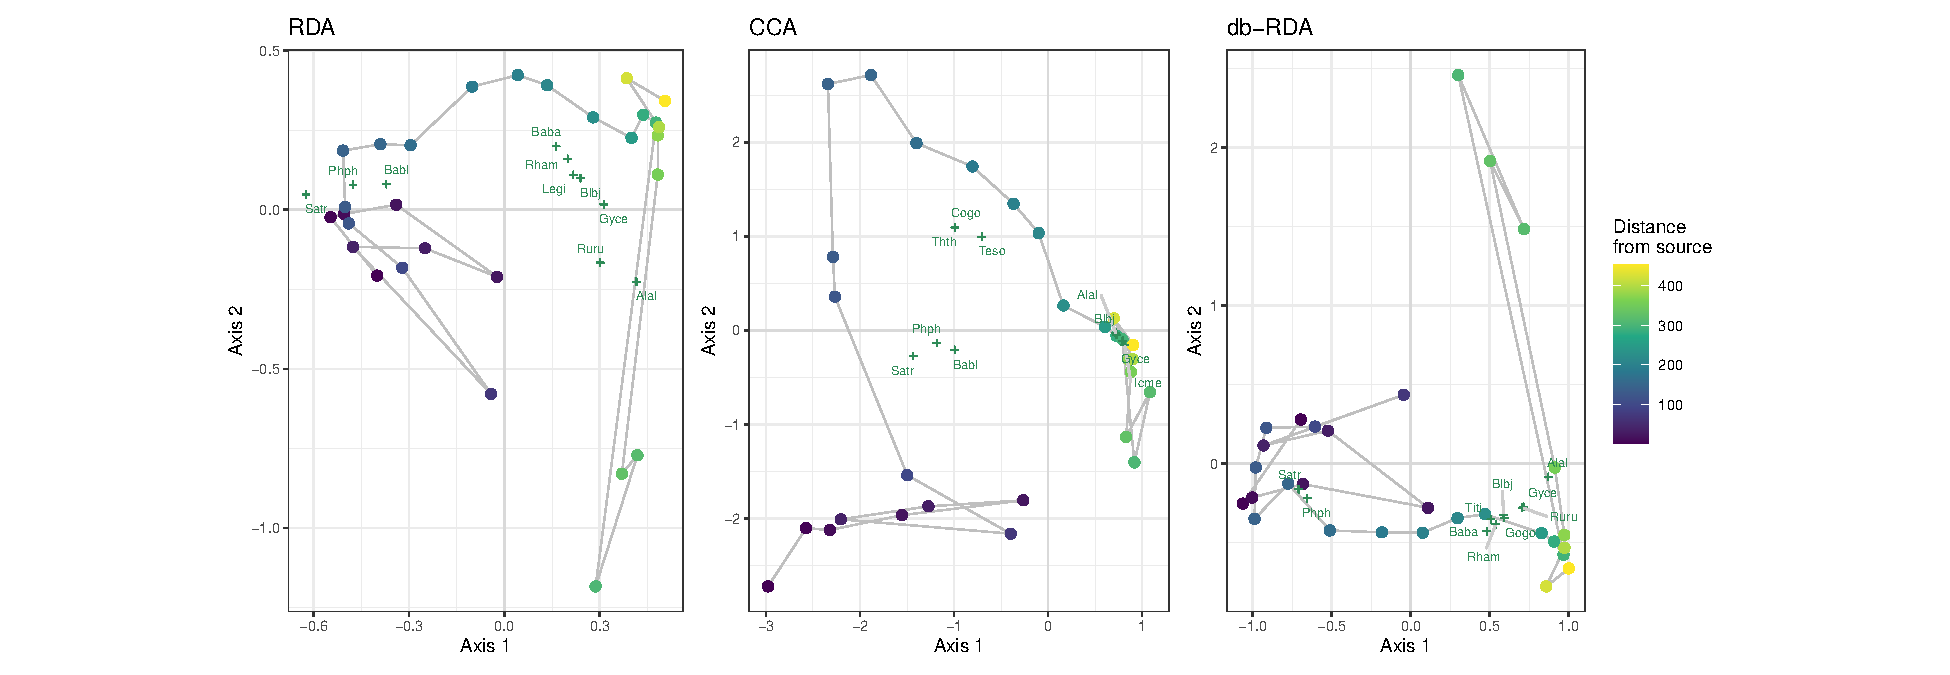
\includegraphics[width=\linewidth]{fig07_constrained_ordination.pdf}
\caption{Selected RDA, CCA, and db-RDA models. Sites are coloured by distance from source.}
\label{fig:constrained}
\end{figure}
\subsection{Data-driven and theory-driven variable selection}
Forward selection is a statistical procedure, not an ecological hypothesis. It keeps whichever variables most improve adjusted $R^2$, and in these data that is \texttt{dfs} together with \texttt{oxy} and \texttt{bod}. A mechanistic reading of the same river suggests a different starting point. Position in the catchment sets the physical template, since altitude and distance from source govern temperature, slope, and discharge. Land use along the valley then loads the water with dissolved inorganic nitrogen (DIN, namely nitrate plus ammonium) and with phosphate. That nutrient load drives primary production and the supply of degradable organic matter, which raises biological oxygen demand, and the respiration that follows draws down dissolved oxygen. In this chain nutrients are the upstream lever and oxygen is a downstream consequence. A researcher who wants the model to name a cause rather than a correlate might therefore prefer a nutrient variable over oxygen, on the grounds that nutrient input is what a catchment manager can actually change.
Table~\ref{tab:tab:theory-compare} puts that intuition to a test. It fits several candidate Hellinger RDA models and compares their adjusted $R^2$ and their worst variance inflation factor. Distance from source alone already reaches adjusted $R^2 = 0.37$. Adding nitrate lifts it only to 0.39, whereas adding oxygen and biological oxygen demand lifts it to 0.54. The two nutrient-loading models, altitude with nitrate and either ammonium or phosphate, settle near 0.39 as well, and their variance inflation factors stay modest. Swapping the enrichment pair for a nutrient variable therefore costs about 0.15 of adjusted $R^2$, which is not a rounding difference.
\begin{table}[!h]
\centering
\caption{\label{tab:tab:theory-compare}Data-driven and theory-driven candidate constrained models, all fitted as Hellinger RDA. Adjusted $R^2$ measures explanatory power and the maximum VIF measures residual collinearity within each candidate set.}
\centering
\resizebox{\ifdim\width>\linewidth\linewidth\else\width\fi}{!}{
\fontsize{8}{10}\selectfont
\begin{tabular}[t]{lllll}
\toprule
Model & Predictors & Rationale & Adjusted R2 & Max VIF\\
\midrule
Forward-selected & \texttt{dfs}, \texttt{oxy}, \texttt{bod} & ordiR2step() data-driven selection & 0.536 & 4.12\\
Position only & \texttt{dfs} & Single longitudinal-position variable & 0.367 & 1.00\\
Position + nitrate & \texttt{dfs}, \texttt{nit} & Position plus the nutrient that tracks the continuum & 0.388 & 2.20\\
Nutrient loading & \texttt{alt}, \texttt{nit}, \texttt{amm} & Altitude plus dissolved inorganic nitrogen & 0.389 & 8.14\\
Nutrient + phosphate & \texttt{alt}, \texttt{nit}, \texttt{pho} & Altitude plus nitrogen and phosphorus loading & 0.383 & 6.32\\
\bottomrule
\end{tabular}}
\end{table}
The reason for that cost is visible in the correlations of Table~\ref{tab:tab:enrich-cor}. Along the clean part of the continuum, oxygen, biological oxygen demand, nitrate, ammonium, and phosphate move together, with many pairwise correlations above 0.7 in absolute value, so any one of them stands in for the others and the choice among them is largely interpretive. The exception is where the ecology becomes interesting. Nitrate rises almost monotonically with distance from source ($r = 0.75$) and tracks the continuum, whereas oxygen and biological oxygen demand decouple from it at the mid-river reach near sites 23 to 25, where oxygen falls to 4 to 6 mg\,L$^{-1}$ and biological oxygen demand exceeds 12 mg\,L$^{-1}$. Forward selection retains oxygen and biological oxygen demand precisely because they carry that local oxygen sag, which a position or nitrate model cannot reproduce.
\begin{table}[!h]
\centering
\caption{\label{tab:tab:enrich-cor}Pearson correlations among distance from source and the enrichment variables across the 29 matched sites. The tight cluster among oxygen, biological oxygen demand, nitrate, ammonium, and phosphate is the collinearity that makes them substitutable along the continuum.}
\centering
\resizebox{\ifdim\width>\linewidth\linewidth\else\width\fi}{!}{
\fontsize{8}{10}\selectfont
\begin{tabular}[t]{lllllll}
\toprule
 & \texttt{dfs} & \texttt{oxy} & \texttt{bod} & \texttt{nit} & \texttt{amm} & \texttt{pho}\\
\midrule
\texttt{dfs} & 1.00 & -0.57 & 0.43 & 0.74 & 0.41 & 0.47\\
\texttt{oxy} & -0.57 & 1.00 & -0.84 & -0.69 & -0.75 & -0.76\\
\texttt{bod} & 0.43 & -0.84 & 1.00 & 0.68 & 0.90 & 0.91\\
\texttt{nit} & 0.74 & -0.69 & 0.68 & 1.00 & 0.80 & 0.80\\
\texttt{amm} & 0.41 & -0.75 & 0.90 & 0.80 & 1.00 & 0.97\\
\texttt{pho} & 0.47 & -0.76 & 0.91 & 0.80 & 0.97 & 1.00\\
\bottomrule
\end{tabular}}
\end{table}
The honest reading is therefore layered. For a management question about nutrient control, DIN is the defensible predictor, and it forfeits little explanatory power over the continuum. For describing the community that is actually present, oxygen is more than a proxy; near the pollution reach it is a proximate stressor with a signal of its own, and dropping it would discard the one place where the river departs from a smooth gradient. Statistical selection cannot arbitrate between these readings, because the variables are collinear over most of the river and diverge only at a handful of sites. The choice is an ecological judgement informed by the correlation structure, not an output of the algorithm. This is the sense in which explanation is not causation: \texttt{ordiR2step()} finds the most economical description of the pattern, but the causal ordering of nutrients, organic load, and oxygen must be supplied by the ecology.
\section{Additional Advanced Analyses}
The analyses in this section sit outside the core Quantitative Ecology chapter sequence. Each re-examines the river-continuum interpretation from an angle the ordinations do not cover, namely the separation of environment from space, the correlation of whole dissimilarity matrices, the decomposition of beta diversity, the identification of ecologically distinctive sites and species, and the shape of individual species responses. They extend the ordinations rather than replace them, and several of them sharpen the interpretation by showing where the smooth-continuum picture breaks down. Table~\ref{tab:tab:advanced-summary} maps the section.
\begin{table}[!h]
\centering
\caption{\label{tab:tab:advanced-summary}Advanced analyses added beyond the core Quantitative Ecology workflow, with their purpose and headline result.}
\centering
\resizebox{\ifdim\width>\linewidth\linewidth\else\width\fi}{!}{
\fontsize{7}{9}\selectfont
\begin{tabular}[t]{lll}
\toprule
Analysis & Purpose & Result\\
\midrule
Variation partitioning & Separate pure environmental, pure spatial, and shared spatial-environmental fractions. & Environment only adj. $R^2$ = 0.106; space only adj. $R^2$ = 0.123\\
MEM spatial eigenvectors & Model spatially structured community variation using Moran eigenvector maps. & MEM2, MEM3, MEM1, MEM4; adj. $R^2$ = 0.551; p = 0.001\\
Procrustes comparison & Compare environmental PCA geometry with fish-community nMDS geometry. & Procrustes r = 0.748; p = 0.001\\
Negative-binomial manyGLM & Test species abundances with a model-based multivariate count framework. & dfs, bod, and oxy p = 0.002, 0.002, 0.002\\
Mantel and partial Mantel & Correlate the fish, environmental, and geographic distance matrices directly. & partial env $|$ space r = 0.564; partial space $|$ env r = 0.177\\
Beta-diversity partitioning & Split total dissimilarity into species replacement and abundance-gradient parts. & turnover = 0.86 of total; gradient = 0.14\\
LCBD and SCBD & Rank sites and species by their contribution to total beta diversity. & 5 sites at p $\leq$ 0.05, incl. headwater and pollution reach\\
Species-response GLMs & Fit abundance responses to distance from source for individual species. & 5 of 8 species unimodal within survey\\
\bottomrule
\end{tabular}}
\end{table}
\subsection{Environment-Space Variation Partitioning}
Variation partitioning splits the Hellinger-transformed community variation into four fractions, namely the part explained uniquely by the selected environmental variables, the part explained uniquely by spatial position, the part they explain jointly, and the unexplained remainder. The exercise is informative here because river environments are spatially organised. Sites further downstream are also further along the channel, so environment and space are confounded by construction, and a large shared fraction is expected rather than a nuisance to be removed. Working through Table~\ref{tab:tab:variation-partition}, the pure environmental fraction is adjusted $R^2 = 0.11$ and the pure spatial fraction is 0.12, while the shared fraction reaches 0.43. Most of the explained community variation is therefore jointly attributable to environment and position, which is the numerical statement of the fact that the environmental gradient is laid out along the length of the river. Only about a third of the variation (adjusted $R^2 = 0.34$) is left unexplained.
\begin{table}[!h]
\centering
\caption{\label{tab:tab:variation-partition}Variation partitioning between selected environmental predictors and polynomial spatial coordinates.}
\centering
\resizebox{\ifdim\width>\linewidth\linewidth\else\width\fi}{!}{
\fontsize{7}{9}\selectfont
\begin{tabular}[t]{llll}
\toprule
Fraction & Interpretation & Adjusted R2 & p\\
\midrule
Environment only & Selected environmental predictors after conditioning on polynomial space & 0.106 & 0.001\\
Space only & Spatial trend after conditioning on selected environmental predictors & 0.123 & 0.001\\
Shared environment-space & Variation jointly structured by measured environment and spatial position & 0.430 & \\
Residual & Unexplained variation & 0.341 & \\
\bottomrule
\end{tabular}}
\end{table}
\subsection{Spatial Eigenvectors, Procrustes Rotation, and manyGLM}
Moran eigenvector maps (MEMs) are orthogonal spatial variables that describe pattern at a range of scales, from a broad upstream-to-downstream trend to finer alternations between neighbouring reaches. Forward selection over the MEM set retains four of them and reaches adjusted $R^2 = 0.55$ ($p = 0.001$), which confirms that the fish assemblage is spatially structured along the river network. The MEMs name no environmental cause. They quantify the scale at which spatial structure exists, and the broadest-scale MEMs carry the same longitudinal signal as distance from source.
The Procrustes rotation asks a geometric question. It rotates and rescales the environmental PCA configuration onto the fish-community nMDS configuration and measures how closely the two point clouds coincide. The fit is strong (Procrustes $r = 0.75$, $p = 0.001$), so a site that is unusual in environmental space tends to be unusual in the same way in faunal space. The two ordinations describe one gradient in two currencies.
The manyGLM analysis moves from distance-based to model-based inference. It fits a negative-binomial generalised linear model to each species, respecting the mean-variance relationship of counts that dissimilarity indices only approximate, and it tests the selected predictors jointly by resampling (Table~\ref{tab:tab:manyglm}). Distance from source, biological oxygen demand, and oxygen are each significant ($p = 0.002$), with distance from source carrying much the largest deviance, 430 against 133 and 112 for the two chemistry terms. A method that makes the count distribution explicit therefore reaches the same ranking as the ordinations, which is reassurance that the pattern does not depend on the Bray-Curtis geometry. The agreement across MEM, Procrustes, and manyGLM supports the main conclusion and repeats the standing caution that environment and space are tightly coupled here.
\begin{table}[!h]
\centering
\caption{\label{tab:tab:manyglm}Negative-binomial manyGLM multivariate tests for the db-RDA selected predictors.}
\centering
\resizebox{\ifdim\width>\linewidth\linewidth\else\width\fi}{!}{
\fontsize{7}{9}\selectfont
\begin{tabular}[t]{lrrll}
\toprule
Term & Residual df & Df diff & Deviance & p\\
\midrule
\texttt{dfs} & 27 & 1 & 430.2 & 0.002\\
\texttt{bod} & 26 & 1 & 133.2 & 0.002\\
\texttt{oxy} & 25 & 1 & 112.2 & 0.002\\
\bottomrule
\end{tabular}}
\end{table}
\subsection{Matrix Correlation with Mantel and Partial Mantel Tests}
The Mantel test correlates two distance matrices directly, without first reducing either to ordination axes. Here it compares the fish Bray-Curtis dissimilarity with a Euclidean distance on the standardised environmental variables, and with the geographic distance between sites (Table~\ref{tab:tab:mantel}). Both simple correlations are significant, but the environmental matrix is much the stronger match (Mantel $r = 0.61$ against $r = 0.32$ for geography). The partial tests then hold one matrix constant while testing the other. Community structure remains strongly tied to environment once geography is held constant ($r = 0.56$, $p = 0.001$), whereas its tie to geography almost disappears once environment is held constant ($r = 0.18$, $p = 0.015$). The environment carries most of the signal, and the pure-space contribution is small. This agrees in direction with the variation partitioning, though the two methods weight the environment differently, since the Mantel test uses the full eleven-variable environmental distance while the partitioning uses only the three selected predictors. Mantel correlations are also known to be conservative and to depend on the distance measure, so they are read as corroboration rather than as a separate estimate of effect size.
\begin{table}[!h]
\centering
\caption{\label{tab:tab:mantel}Mantel and partial Mantel correlations among the fish, environmental, and geographic distance matrices, with 999 permutations.}
\centering
\resizebox{\ifdim\width>\linewidth\linewidth\else\width\fi}{!}{
\fontsize{8}{10}\selectfont
\begin{tabular}[t]{lll}
\toprule
Test & Mantel r & p\\
\midrule
Community vs environment & 0.606 & 0.001\\
Community vs geographic distance & 0.319 & 0.001\\
Community vs environment, geography held constant & 0.564 & 0.001\\
Community vs geography, environment held constant & 0.177 & 0.015\\
\bottomrule
\end{tabular}}
\end{table}
\subsection{Beta-Diversity Components: Replacement and Abundance Gradient}
The central claim of the report is that downstream change is a replacement of one set of species by another rather than a simple loss of species. Beta-diversity partitioning tests that claim quantitatively by splitting the total multi-site Bray-Curtis dissimilarity into a balanced-variation component, which is true turnover where a gain of one species is matched by a loss of another, and an abundance-gradient component, which is the nestedness-like part where assemblages differ because one is a subset or a diluted version of the other (Table~\ref{tab:tab:betapart}). Turnover dominates. It accounts for 0.86 of the total dissimilarity, against 0.14 for the abundance-gradient component. The pattern is therefore replacement, which is consistent with the long DCA gradient and with the species arch in the CA. The abundance-gradient component is not zero, and the sites that inflate it are the depauperate ones at the two ends of the disturbance range, namely the headwater and the polluted mid-river reach, where the assemblage is a thinned subset of the richer lowland fauna rather than a distinct set of species. Beta-diversity partitioning thus recovers both processes and shows which one dominates.
\begin{table}[!h]
\centering
\caption{\label{tab:tab:betapart}Multi-site beta-diversity partitioning of the fish assemblage into balanced turnover and abundance-gradient components (Baselga family, abundance-based).}
\centering
\resizebox{\ifdim\width>\linewidth\linewidth\else\width\fi}{!}{
\fontsize{8}{10}\selectfont
\begin{tabular}[t]{lll}
\toprule
Component & Value & Share of total\\
\midrule
Total dissimilarity (beta.BRAY) & 0.909 & 1.000\\
Balanced turnover (species replacement) & 0.779 & 0.857\\
Abundance gradient (nestedness-like) & 0.130 & 0.143\\
\bottomrule
\end{tabular}}
\end{table}
\subsection{Distinctive Sites and Species: LCBD and SCBD}
Local contributions to beta diversity (LCBD) rank the sites by how much each one adds to the total variance of the community matrix, and species contributions (SCBD) do the same for the species. High-LCBD sites are ecologically distinctive, whether through rarity, unusual composition, or a departure from the general trend. Table~\ref{tab:tab:lcbd} lists the six sites with the largest LCBD, and the permutation p-values flag those whose distinctiveness exceeds chance. The result is telling. The most distinctive sites are the extreme headwater (site 1, a near-monospecific brown-trout reach) and the organic-pollution zone (sites 23 to 25), each significant at $p \leq 0.05$. These are exactly the two places where the smooth continuum is interrupted, the first by the severity of the upstream physical filter and the second by the mid-river oxygen sag. The heaviest SCBD contributions come from the gradient-defining species, led by 
\texttt{Satr} (Brown trout, 0.142), \texttt{Phph} (Minnow, 0.095), \texttt{Alal} (Bleak, 0.080), \texttt{Babl} (Stone loach, 0.071), \texttt{Ruru} (Roach, 0.055). Figure~\ref{fig:lcbd} places the LCBD values and the site-level species richness along distance from source, and the richness collapse at sites 23 to 25, from 22 species down to 3, coincides with the LCBD peak there.
\begin{table}[!h]
\centering
\caption{\label{tab:tab:lcbd}The six sites with the largest local contribution to beta diversity (LCBD), with distance from source and the permutation p-value.}
\centering
\resizebox{\ifdim\width>\linewidth\linewidth\else\width\fi}{!}{
\fontsize{8}{10}\selectfont
\begin{tabular}[t]{rlll}
\toprule
Site & Distance from source & LCBD & p\\
\midrule
1 & 0.3 & 0.0725 & 0.001\\
23 & 304.3 & 0.0616 & 0.001\\
24 & 314.7 & 0.0524 & 0.011\\
13 & 143.6 & 0.0477 & 0.044\\
25 & 327.8 & 0.0476 & 0.037\\
2 & 2.2 & 0.0445 & 0.094\\
\bottomrule
\end{tabular}}
\end{table}
\begin{figure}[H]
\centering
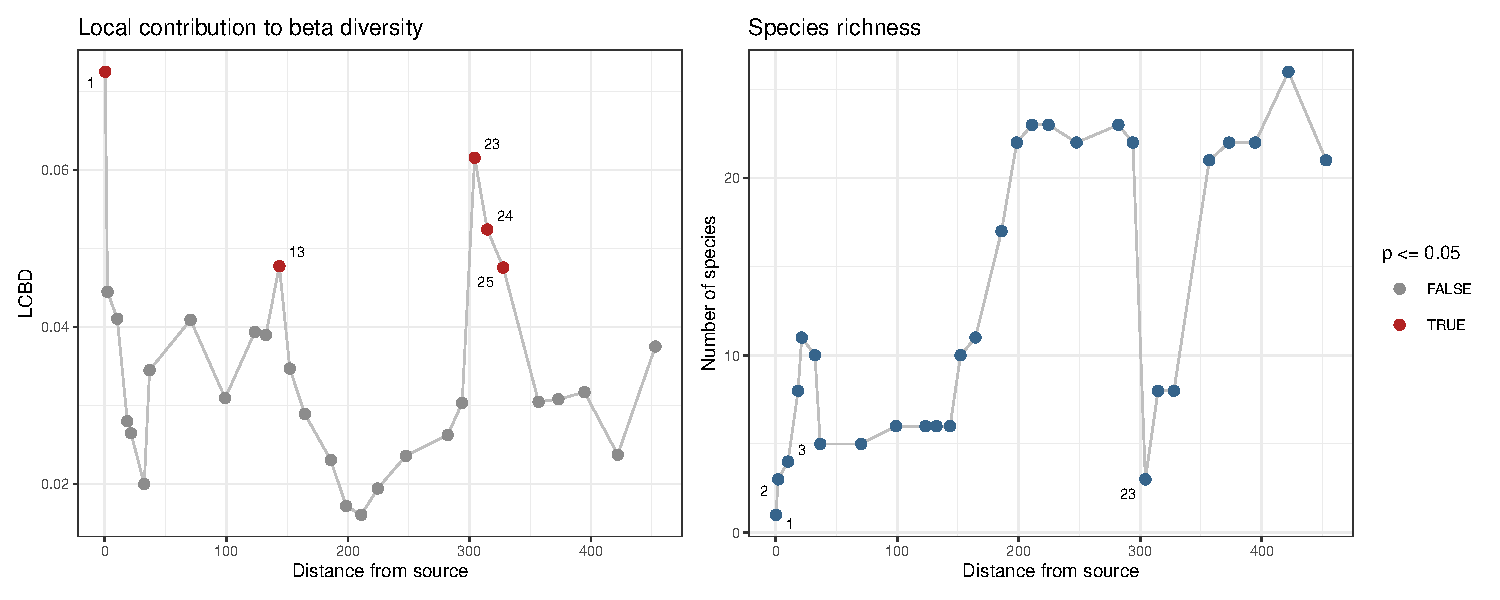
\includegraphics[width=\linewidth]{fig10_lcbd_richness.pdf}
\caption{Local contribution to beta diversity (left) and species richness (right) along distance from source. Firebrick points on the left mark sites significant at $p \leq 0.05$; the richness minimum at sites 23 to 25 marks the organic-pollution reach.}
\label{fig:lcbd}
\end{figure}
\subsection{Species-Response Shapes Along the Gradient}
The ordinations assume, through the chi-square and Bray-Curtis geometries, that species rise and fall along the gradient rather than increasing without limit. A direct way to check that assumption is to fit each species against distance from source with a negative-binomial generalised linear model that includes a linear and a quadratic term, \texttt{glm.nb(y \textasciitilde{} dfs + I(dfs\textasciicircum{}2))}. A significant negative quadratic term indicates a unimodal response with an optimum inside the surveyed reach, and the optimum itself is the fitted peak position (Table~\ref{tab:tab:response}, Figure~\ref{fig:response}). Headwater and mid-river species show clear unimodal responses with optima ordered along the channel, from brown trout near 50 km through stone loach, bullhead, and grayling to barbel near 350 km. The lowland species behave differently. Roach, gudgeon, and common bream are still rising at the downstream end of the survey, so their fitted optima lie beyond the sampled reach and their responses are monotonic within it. This is the expected signature of a gradient sampled from its cold, species-poor source to a lower reach that has not yet reached the true lowland optima of the most downstream taxa, and it is the same truncation that gives the DCA its long first axis.
\begin{table}[!h]
\centering
\caption{\label{tab:tab:response}Negative-binomial species-response models against distance from source. The fitted optimum is the peak of the quadratic response where it falls inside the surveyed reach; the quadratic p-value tests for curvature.}
\centering
\resizebox{\ifdim\width>\linewidth\linewidth\else\width\fi}{!}{
\fontsize{8}{10}\selectfont
\begin{tabular}[t]{lllll}
\toprule
Code & Species & Fitted optimum (km) & Quadratic p & Response\\
\midrule
\texttt{Satr} & Brown trout & 53 & 0.022 & Unimodal, optimum within survey\\
\texttt{Cogo} & Bullhead & 163 & 0.020 & Unimodal, optimum within survey\\
\texttt{Thth} & Grayling & 182 & 0.016 & Unimodal, optimum within survey\\
\texttt{Babl} & Stone loach & 99 & 0.010 & Unimodal, optimum within survey\\
\texttt{Baba} & Barbel & 348 & 0.017 & Unimodal, optimum within survey\\
\texttt{Gogo} & Gudgeon & beyond survey & 0.317 & Increasing, optimum below survey\\
\texttt{Ruru} & Roach & beyond survey & 0.979 & Increasing, optimum below survey\\
\texttt{Abbr} & Common bream & beyond survey & 0.200 & Increasing, optimum below survey\\
\bottomrule
\end{tabular}}
\end{table}
\begin{figure}[H]
\centering
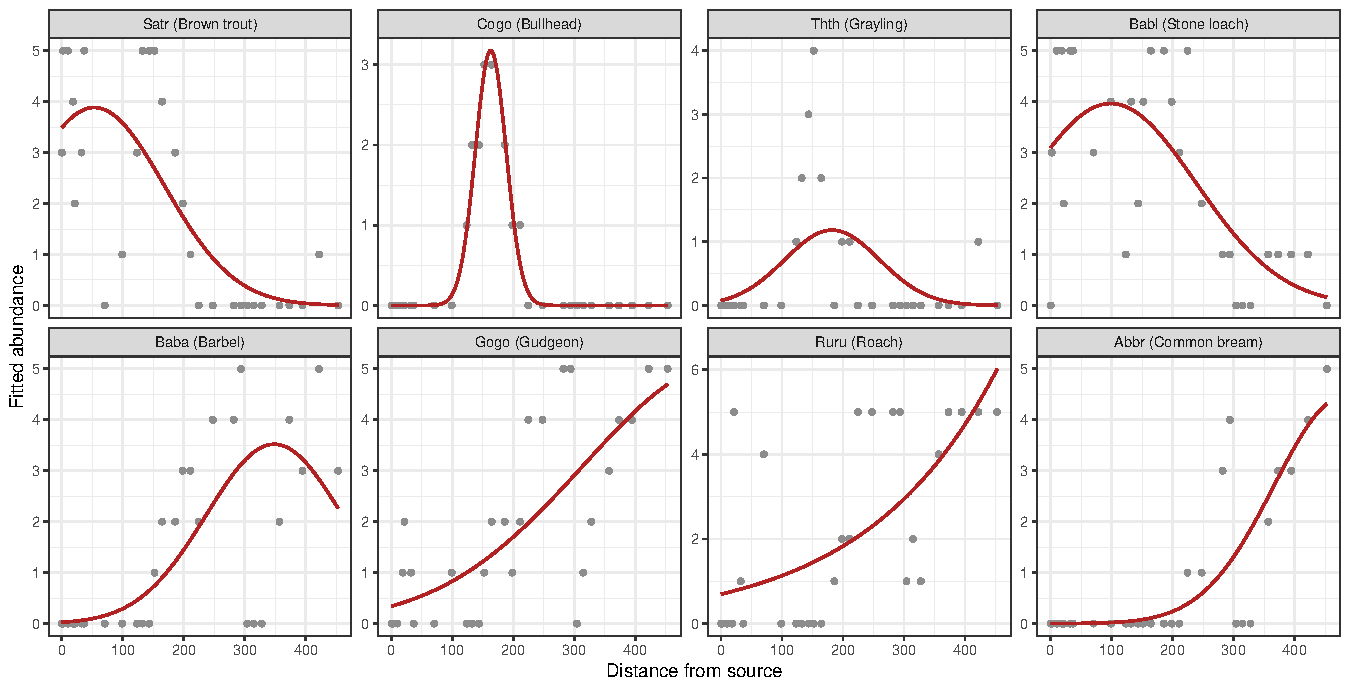
\includegraphics[width=\linewidth]{fig09_species_response.pdf}
\caption{Fitted negative-binomial abundance responses (firebrick) with observed counts (grey) against distance from source, for species spanning the gradient. Vertical scales differ between panels.}
\label{fig:response}
\end{figure}
\section{Species Replacement Along the Gradient}
The ordinations reduce the data to axes. The raw abundance pattern shows the ecological turnover directly (Figure~\ref{fig:species-gradient}). The gradient has a physical origin. Near the source the channel is high, steep, and cold, the discharge is low but turbulent, and the water is close to oxygen saturation. Downstream the profile flattens, discharge and hardness rise, the water warms, and organic matter accumulates and decays over a longer residence time. This physical template sets up a chemical one, since warmer, slower, nutrient-richer water supports more production and a higher biological oxygen demand. The fish assemblage is layered onto both.
Each species occupies a bounded stretch of the gradient, and the stretches are ordered, which is what produces replacement rather than simple enrichment or loss. The headwaters hold cool-water specialists, namely brown trout, bullhead, minnow, and grayling, whose fitted optima fall in the upper reaches (Table~\ref{tab:tab:response}). Stone loach and barbel take over through the middle river. The lower reaches are held by cyprinids and generalists such as roach, common bream, bleak, and eel, whose abundances are still climbing at the downstream limit of the survey. The sequence recovers the classical river fish zonation, from a trout zone through grayling and barbel zones to a bream zone, expressed as a continuous replacement rather than a set of sharp boundaries.
One reach departs from the smooth sequence. At sites 23 to 25 the water chemistry changes abruptly, with biological oxygen demand rising above 12 mg\,L$^{-1}$, ammonium reaching 1.8 mg\,L$^{-1}$, and dissolved oxygen falling to 4 to 6 mg\,L$^{-1}$. This is the chemical signature of a point-source organic load. Species richness collapses from 22 at site 22 to 3 at site 23 before recovering downstream (Figure~\ref{fig:lcbd}), and these sites carry the highest local contributions to beta diversity outside the headwater. The organic-pollution reach is a second, shorter gradient superimposed on the longitudinal one, an oxygen sag that thins the assemblage locally and then releases it as the river re-aerates. This reach is what keeps oxygen and biological oxygen demand in the selected constrained models and what lifts the abundance-gradient component of beta diversity above zero.
\begin{figure}[H]
\centering
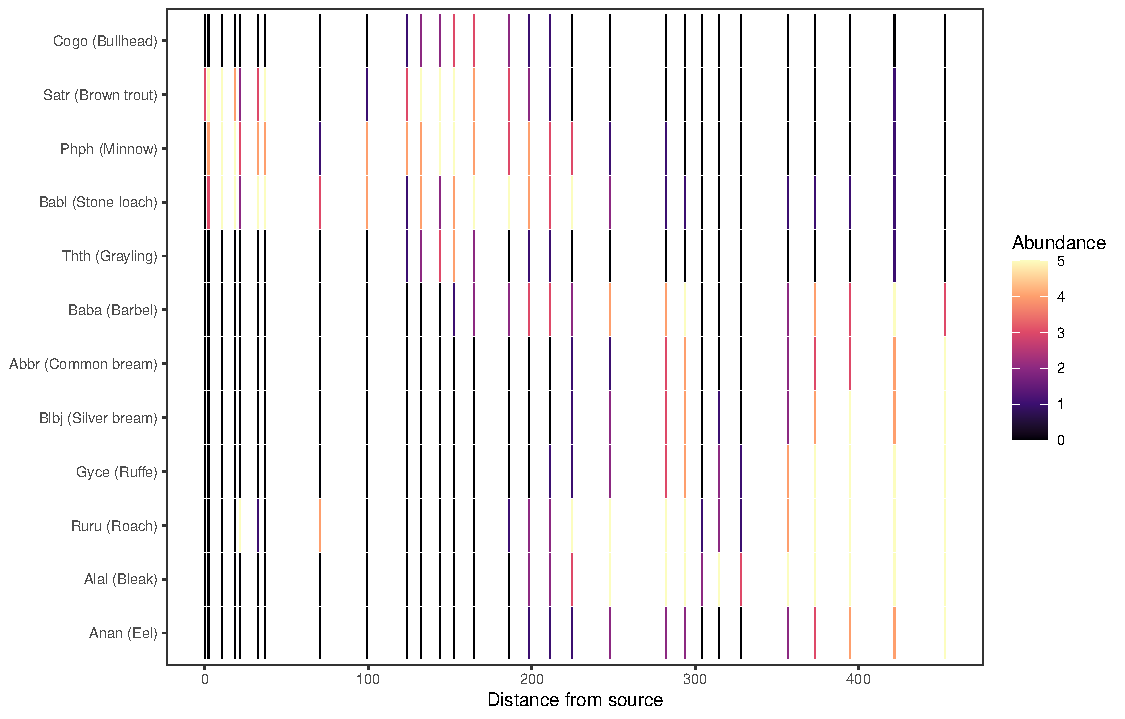
\includegraphics[width=0.95\linewidth]{fig08_species_gradient_heatmap.pdf}
\caption{Abundance of representative fish species along distance from source. Species are ordered to show the broad upstream-to-downstream replacement.}
\label{fig:species-gradient}
\end{figure}
\section{Discussion: Gradients that Structure the System}
The Doubs assemblage is organised first and foremost by a longitudinal river-continuum gradient. The upper sites are high, steep, cool reaches with near-saturated oxygen and little nutrient or organic load. The lower sites are further from source and lower in altitude, with greater discharge, harder water, more nutrients, and higher biological oxygen demand. These variables correlate because they are different measurements of one downstream integration of catchment, geomorphological, and biogeochemical processes, and every analysis in this report, unconstrained or constrained, distance-based or model-based, recovers that single axis as the dominant structure.
The fish assemblage is layered onto this template as an ordered replacement. The upstream end supports trout-zone species, and downstream those decline and give way to cyprinids and generalists of the warmer, slower, more productive lower river. Because each species occupies a bounded stretch of the gradient (Table~\ref{tab:tab:response}), the turnover is genuine replacement rather than progressive enrichment, which the beta-diversity partitioning confirms by attributing 0.86 of total dissimilarity to balanced turnover. CA, PCoA, and nMDS recover the same sequence from composition alone, so the interpretation rests on the data rather than on one ordination geometry.
The continuum is not perfectly smooth. A short reach at sites 23 to 25 carries a strong organic-load signal, with biological oxygen demand above 12 mg\,L$^{-1}$ and oxygen down to 4 mg\,L$^{-1}$, and the fauna there thins to a few tolerant species before recovering downstream. This reach is the most distinctive part of the river after the headwater on the LCBD ranking, it supplies most of the nestedness-like component of beta diversity, and it is the reason oxygen and biological oxygen demand survive forward selection where nitrate, which tracks the continuum more faithfully, does not. Read together, the analyses describe two overlaid gradients, a long physical-chemical continuum and a short, sharp oxygen sag, rather than a single monotonic trend.
The second ordination axes reward caution. CA2 in particular is partly the arch effect of a long first gradient rather than a separate ecological process, and DCA supports that reading with a first-axis length of 3.9 standard-deviation units. Where second-axis structure is genuine, it is best interpreted as local departure from the main sequence, and the oxygen-sag reach is the clearest example.
The constrained models show that the measured environment explains about half of the community variation, yet they cannot rank the predictors causally, because those predictors are correlated expressions of river position and organic load. Forward selection returns the most economical description, namely distance from source with oxygen and biological oxygen demand, while a mechanistic account would place dissolved inorganic nitrogen upstream of the oxygen response. The two views are compatible. Statistics identifies the compact set of correlates, and ecology supplies the causal ordering. Neither on its own licenses a claim that a single variable drives the fish community.
The analyses are correlational, so association is not mechanism. The gradient is truncated at both ends, so the optima of the most downstream species lie beyond the survey and the headwater is sampled to near-zero richness. Environment and space are confounded along a single channel, so the pure environmental and pure spatial fractions are both small while the shared fraction is large. These are properties of a one-dimensional river surveyed once, and they would be relaxed only by sampling more rivers, more seasons, or by manipulative work.
\section{Reproducibility}
This report was generated by \texttt{BCB743/reports/make\_doubs\_multivariate\_report.R}. The run used \textsf{vegan} 2.7.5 under R 4.5.3, with 999 permutations for the ordination and matrix tests. The advanced analyses used \textsf{adespatial} 0.3.29, \textsf{betapart} 1.6.1, \textsf{mvabund} 4.2.8, \textsf{MASS} 7.3.65. All stochastic steps were seeded with \texttt{set.seed(743)}.
\end{document}
